\chapter{Conception fonctionnelle et technique}

Ce chapitre présente l’ensemble de la conception fonctionnelle et technique du projet. Cette phase constitue un pilier fondamental de la réussite du système, car elle permet d’anticiper les contraintes, de structurer les choix techniques et de sécuriser le développement avant toute implémentation.

La conception a été menée de manière rigoureuse et progressive afin de garantir la cohérence globale du système, la maintenabilité du code et l’adéquation avec les besoins métier identifiés.
\newline

\begin{for_you}{Pourquoi la phase de conception est déterminante}
\begin{itemize}
    \item \textbf{Réduction des coûts de refactorisation} : Une architecture bien pensée limite les reprises de code
    \item \textbf{Pilotage du développement} : Chaque fonctionnalité est clairement définie avant implémentation
    \item \textbf{Facilitation des tests} : Les cas d’usage servent de base aux scénarios de test
    \item \textbf{Maîtrise des risques} : Les problèmes techniques et fonctionnels sont identifiés en amont
    \item \textbf{Amélioration de la communication} : Une vision commune est partagée entre tous les acteurs
\end{itemize}

\textbf{\newline}
\textbf{Contenu du chapitre :}
\begin{itemize}
    \item \mycheckmark Diagrammes de cas d’usage (Use Cases) validés
    \item \mycheckmark Diagrammes de séquence pour les flux critiques
    \item \mycheckmark Modélisation des données (MCD, MLD, MPD)
    \item \mycheckmark Architecture technique justifiée
    \item \mycheckmark User stories avec critères d’acceptation
    \item \mycheckmark Wireframes et maquettes validés
    \item \mycheckmark Charte graphique cohérente
    \item \mycheckmark Stratégie de tests définie
\end{itemize}
\end{for_you}

\section{Cas d’usage et modélisation UML}
Les cas d’usage modélisent les interactions entre les acteurs et le système afin d’identifier précisément les fonctionnalités attendues. Cette approche centrée utilisateur garantit une adéquation directe entre les besoins métier et les fonctionnalités implémentées.
Les diagrammes UML constituent un support de communication essentiel entre les parties prenantes techniques et fonctionnelles, réduisant les risques d’ambiguïté et d’interprétation.

\begin{for_you}{Diagramme de cas d'usage simplifié :}
    \begin{center}
    
\includegraphics[width=15cm,height=80mm]{./assets/uml/diagramme_de_cas_d'utilisation.png}
    \end{center}
\end{for_you}

\section{Diagrammes de séquence}
Les diagrammes de séquence décrivent les interactions temporelles entre les composants du système pour chaque cas d’usage critique. Ils permettent d’identifier clairement les responsabilités de chaque couche de l’architecture 3 tiers.
Cette modélisation facilite l’implémentation des flux, la gestion des erreurs et la conception des tests d’intégration.
\newline

\begin{for_you}{Diagramme de séquence accès site :}
    \begin{center}
        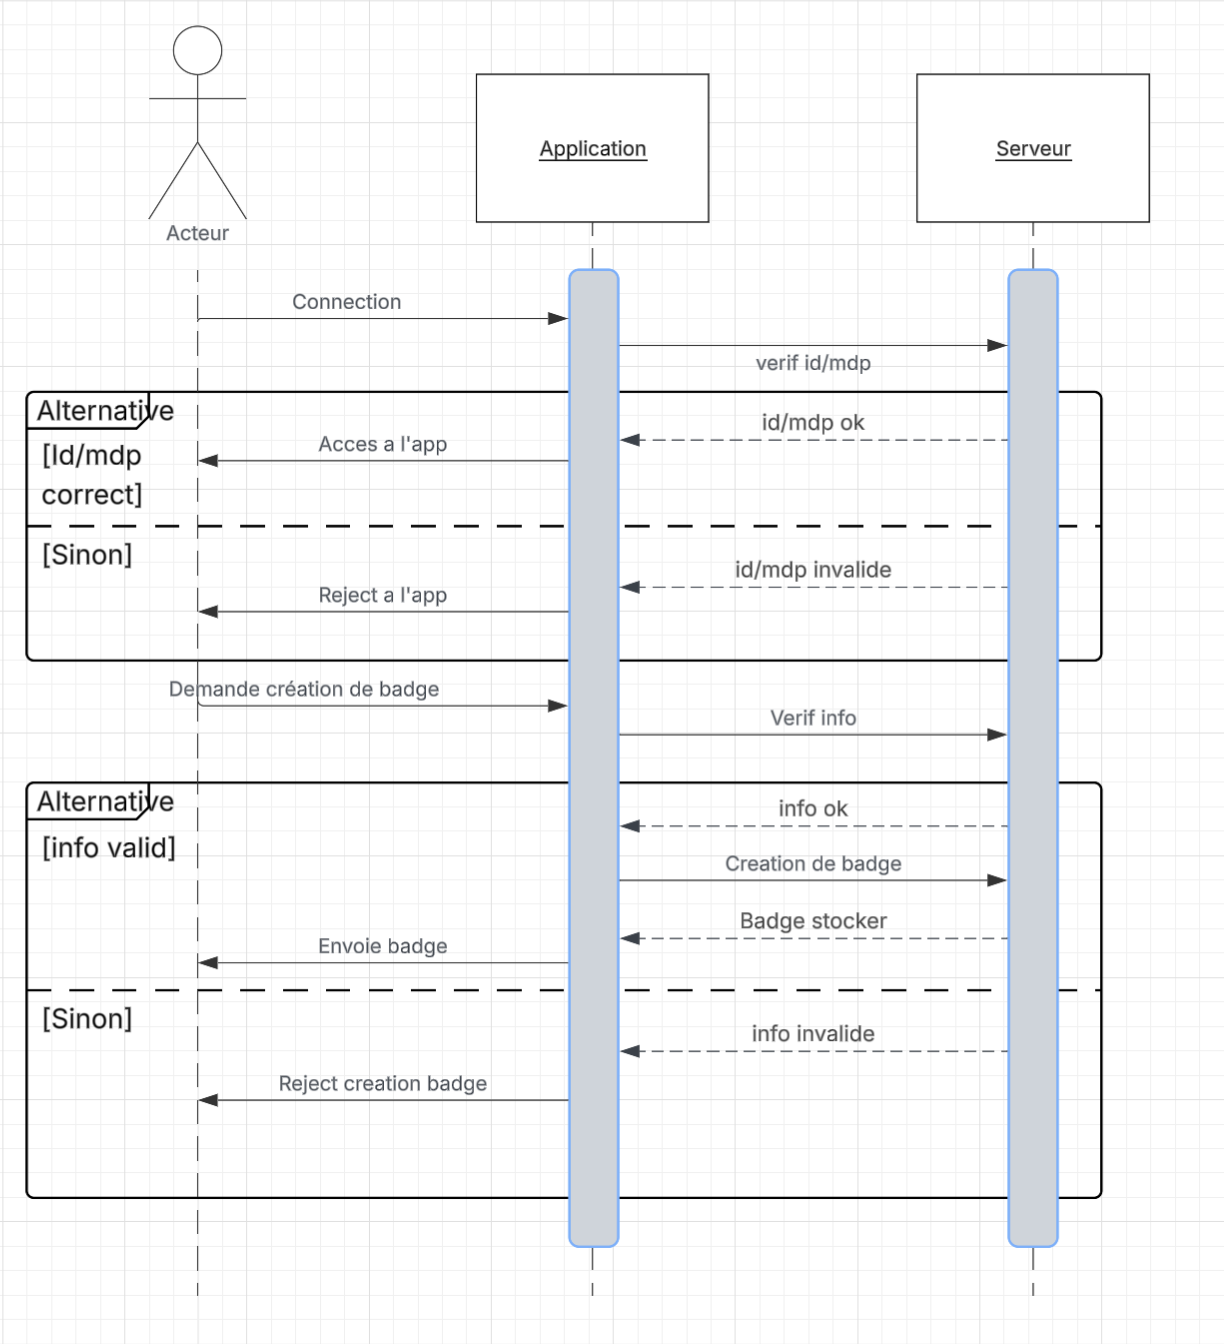
\includegraphics[width=10cm,height=80mm]{./assets/uml/diagramme_de_sequence_acces_site.png}
    \end{center}
\end{for_you}

\begin{for_you}{Diagramme de séquence accès bâtiment :}
    \begin{center}
        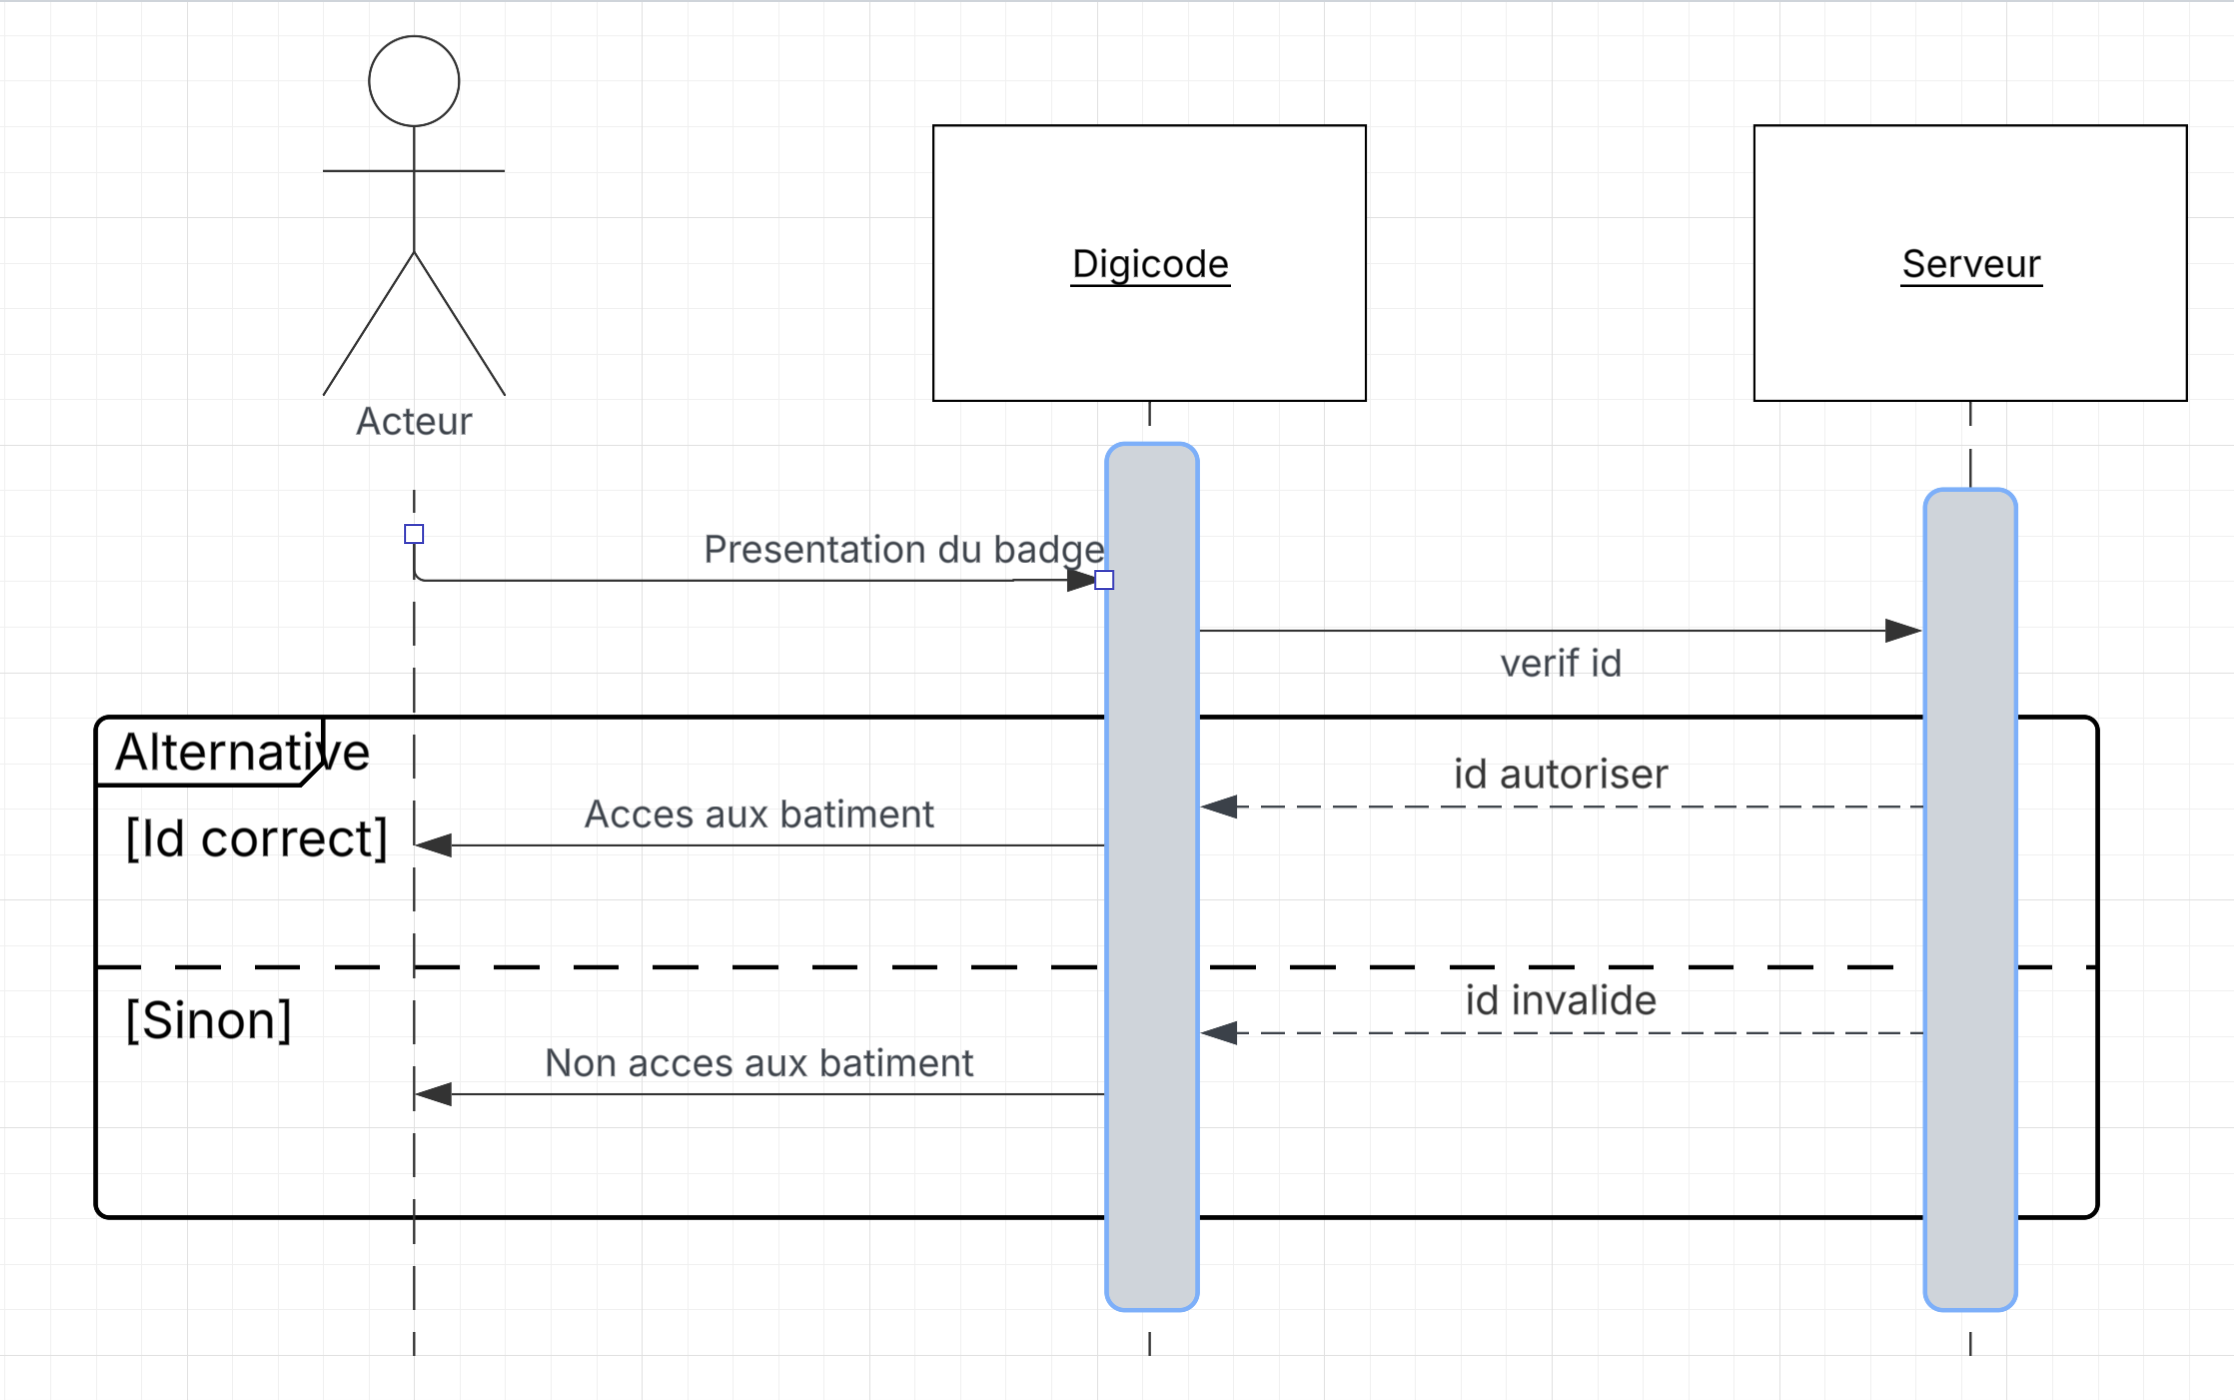
\includegraphics[width=10cm,height=80mm]{./assets/uml/diagramme_de_sequence_acces_batiment.png}
    \end{center}
\end{for_you}

\section{Conception de l’interface utilisateur}
La conception de l’interface repose sur une démarche progressive : zoning, wireframes puis maquettes haute fidélité. Cette méthode permet de valider l’expérience utilisateur avant toute implémentation technique.
L’UX a été pensée pour favoriser la simplicité, la lisibilité et l’efficacité, afin de réduire la courbe d’apprentissage et d’optimiser l’adoption du système.

\subsection{Zoning}
Dans cette sous-section, je vais vous présenter l'organisation spatiale de mes interfaces. Nous verrons une analyse claire de la hiérarchie visuelle et de l'organisation des éléments.
\newline

\begin{for_you}{Page de connexion}
    \begin{center}
        
\includegraphics[width=15cm,height=80mm]{./assets/zoning/page_de_connexion.png}
    \end{center}
\end{for_you}

\textbf{\newline}

\begin{for_you}{Dashboard}
    \begin{center}
        
\includegraphics[width=15cm,height=80mm]{./assets/zoning/dashboard.png}
    \end{center}
\end{for_you}

\textbf{\newline}

\begin{for_you}{Page de gestions d'utilisateur}
    \begin{center}
        
\includegraphics[width=15cm,height=80mm]{./assets/zoning/page_utilisateur.png}
    \end{center}
\end{for_you}

\textbf{\newline}

\begin{for_you}{Page de gestions de badges}
    \begin{center}
        
\includegraphics[width=15cm,height=80mm]{./assets/zoning/page_badge.png}
    \end{center}
\end{for_you}

\textbf{\newline}

\begin{for_you}{Page profil}
    \begin{center}
        
\includegraphics[width=15cm,height=80mm]{./assets/zoning/page_profil.png}
    \end{center}
\end{for_you}

\subsection{Wireframe}

Dans cette sous-section, je vais vous présenter mes wireframes pour les pages principales. Nous verrons une représentation claire de la structure et des interactions.
\newline

\begin{for_you}{Page de connexion}
    \begin{center}
        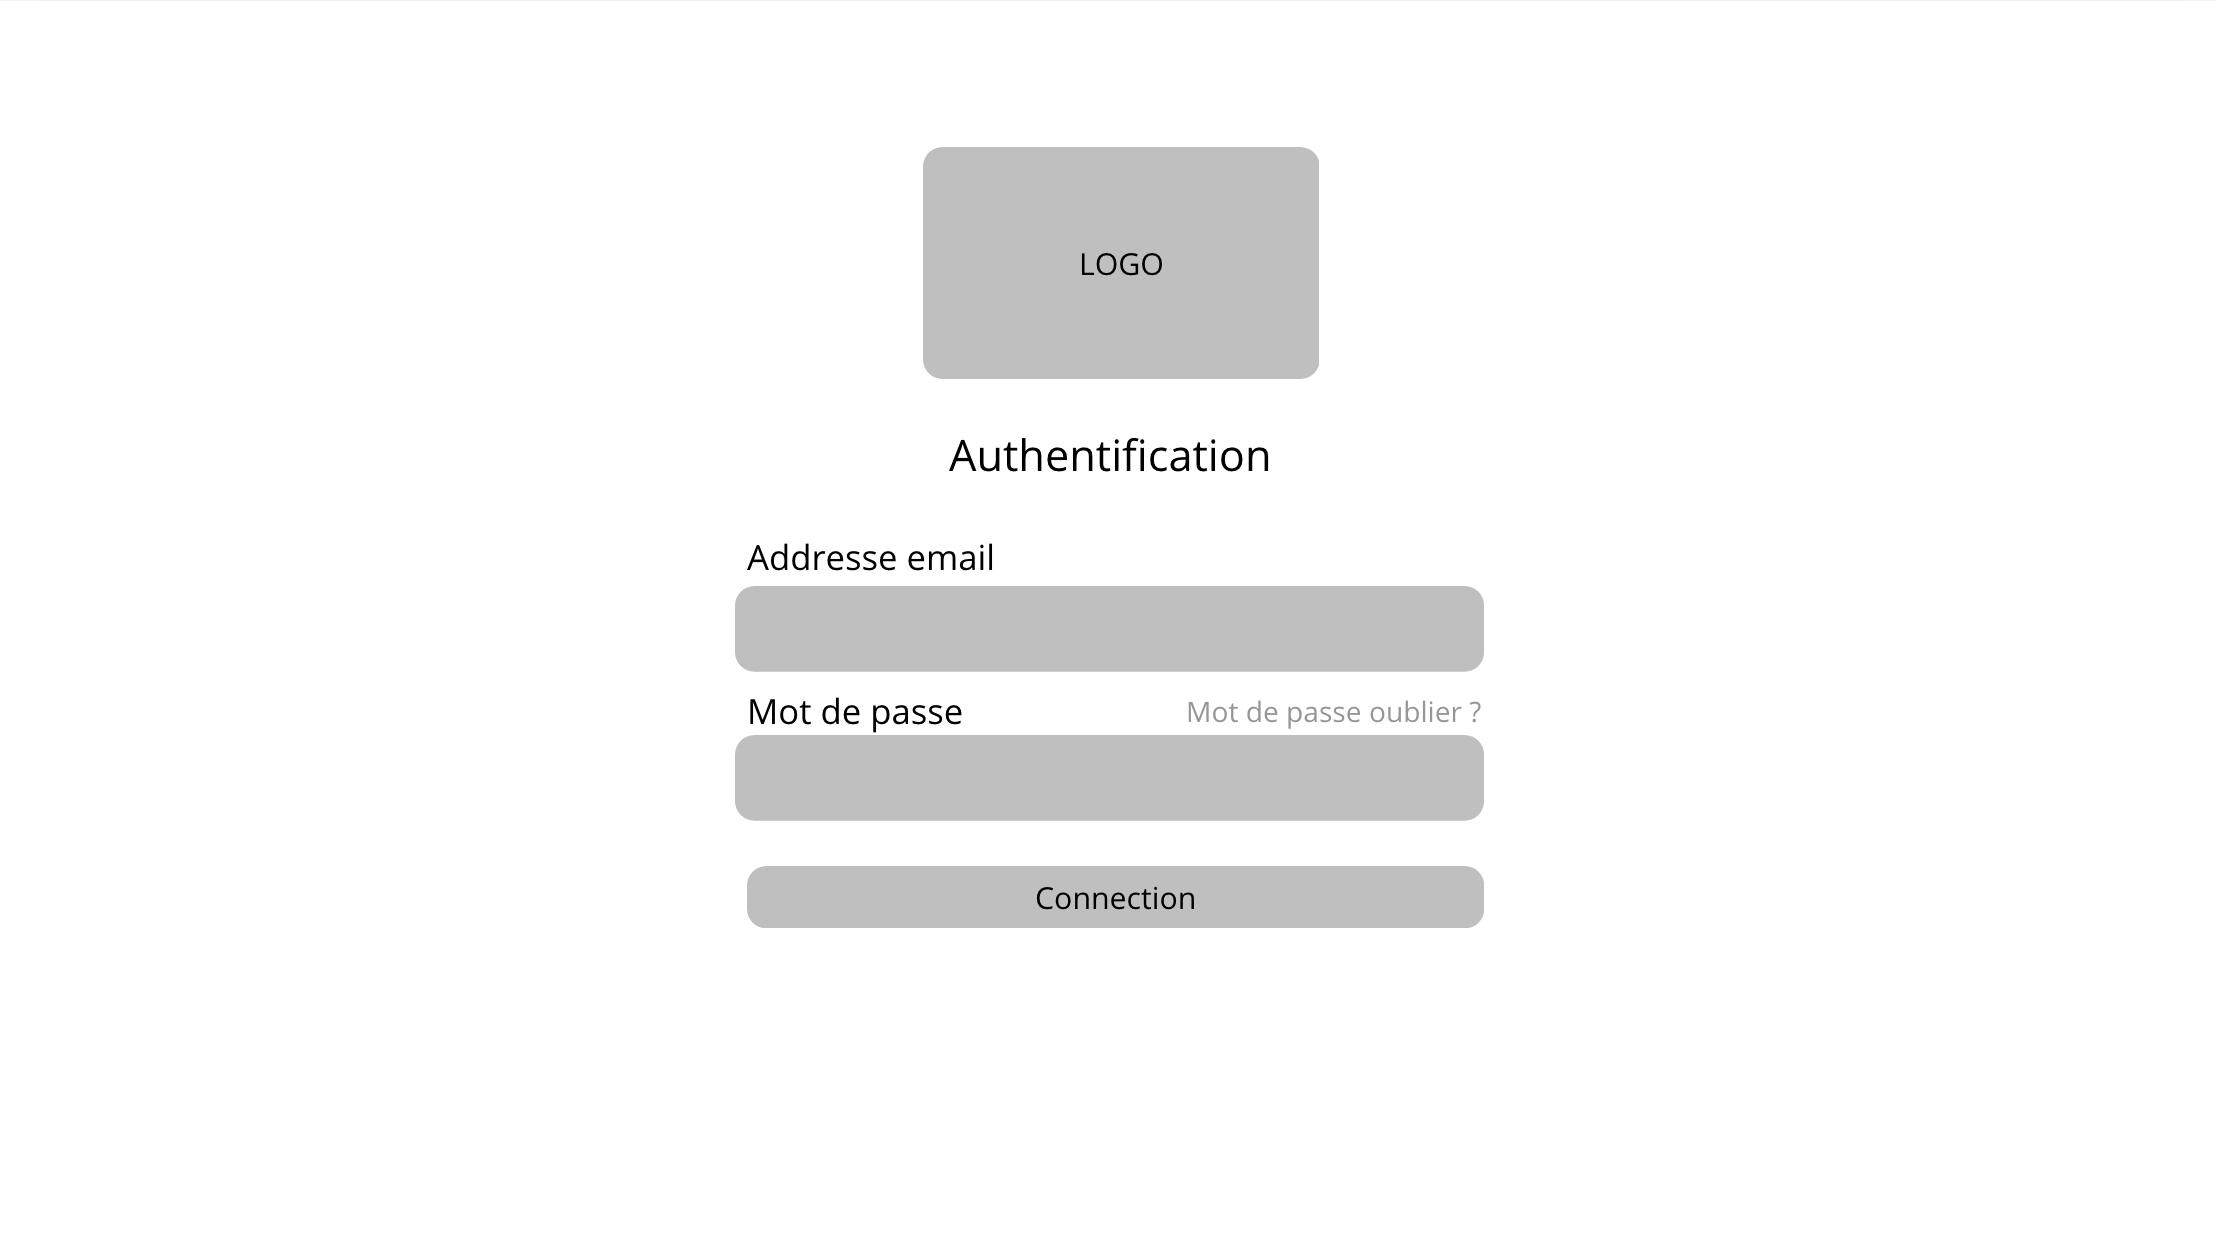
\includegraphics[width=15cm,height=80mm]{./assets/wireframe/page_de_connexion.png}
    \end{center}
\end{for_you}

\textbf{\newline}

\begin{for_you}{Dashboard}
    \begin{center}
        
\includegraphics[width=15cm,height=80mm]{./assets/wireframe/dashboard.png}
    \end{center}
\end{for_you}

\textbf{\newline}

\begin{for_you}{Page de gestions d'utilisateur}
    \begin{center}
        
\includegraphics[width=15cm,height=80mm]{./assets/wireframe/page_utilisateur.png}
    \end{center}
\end{for_you}

\textbf{\newline}

\begin{for_you}{Page de gestions de badges}
    \begin{center}
        
\includegraphics[width=15cm,height=80mm]{./assets/wireframe/page_badge.png}
    \end{center}
\end{for_you}

\textbf{\newline}

\begin{for_you}{Page profil}
    \begin{center}
        
\includegraphics[width=15cm,height=80mm]{./assets/wireframe/page_profil.png}
    \end{center}
\end{for_you}

\subsection{Maquettage}

Dans cette sous-section, je vais vous présenter mes maquettes. Nous verrons une représentation visuelle fidèle au rendu final.

\begin{for_you}{Page de connexion}
    \begin{center}
        
\includegraphics[width=15cm,height=80mm]{./assets/maquette/page_de_conextion.png}
    \end{center}
\end{for_you}

\textbf{\newline}

\begin{for_you}{Dashboard}
    \begin{center}
        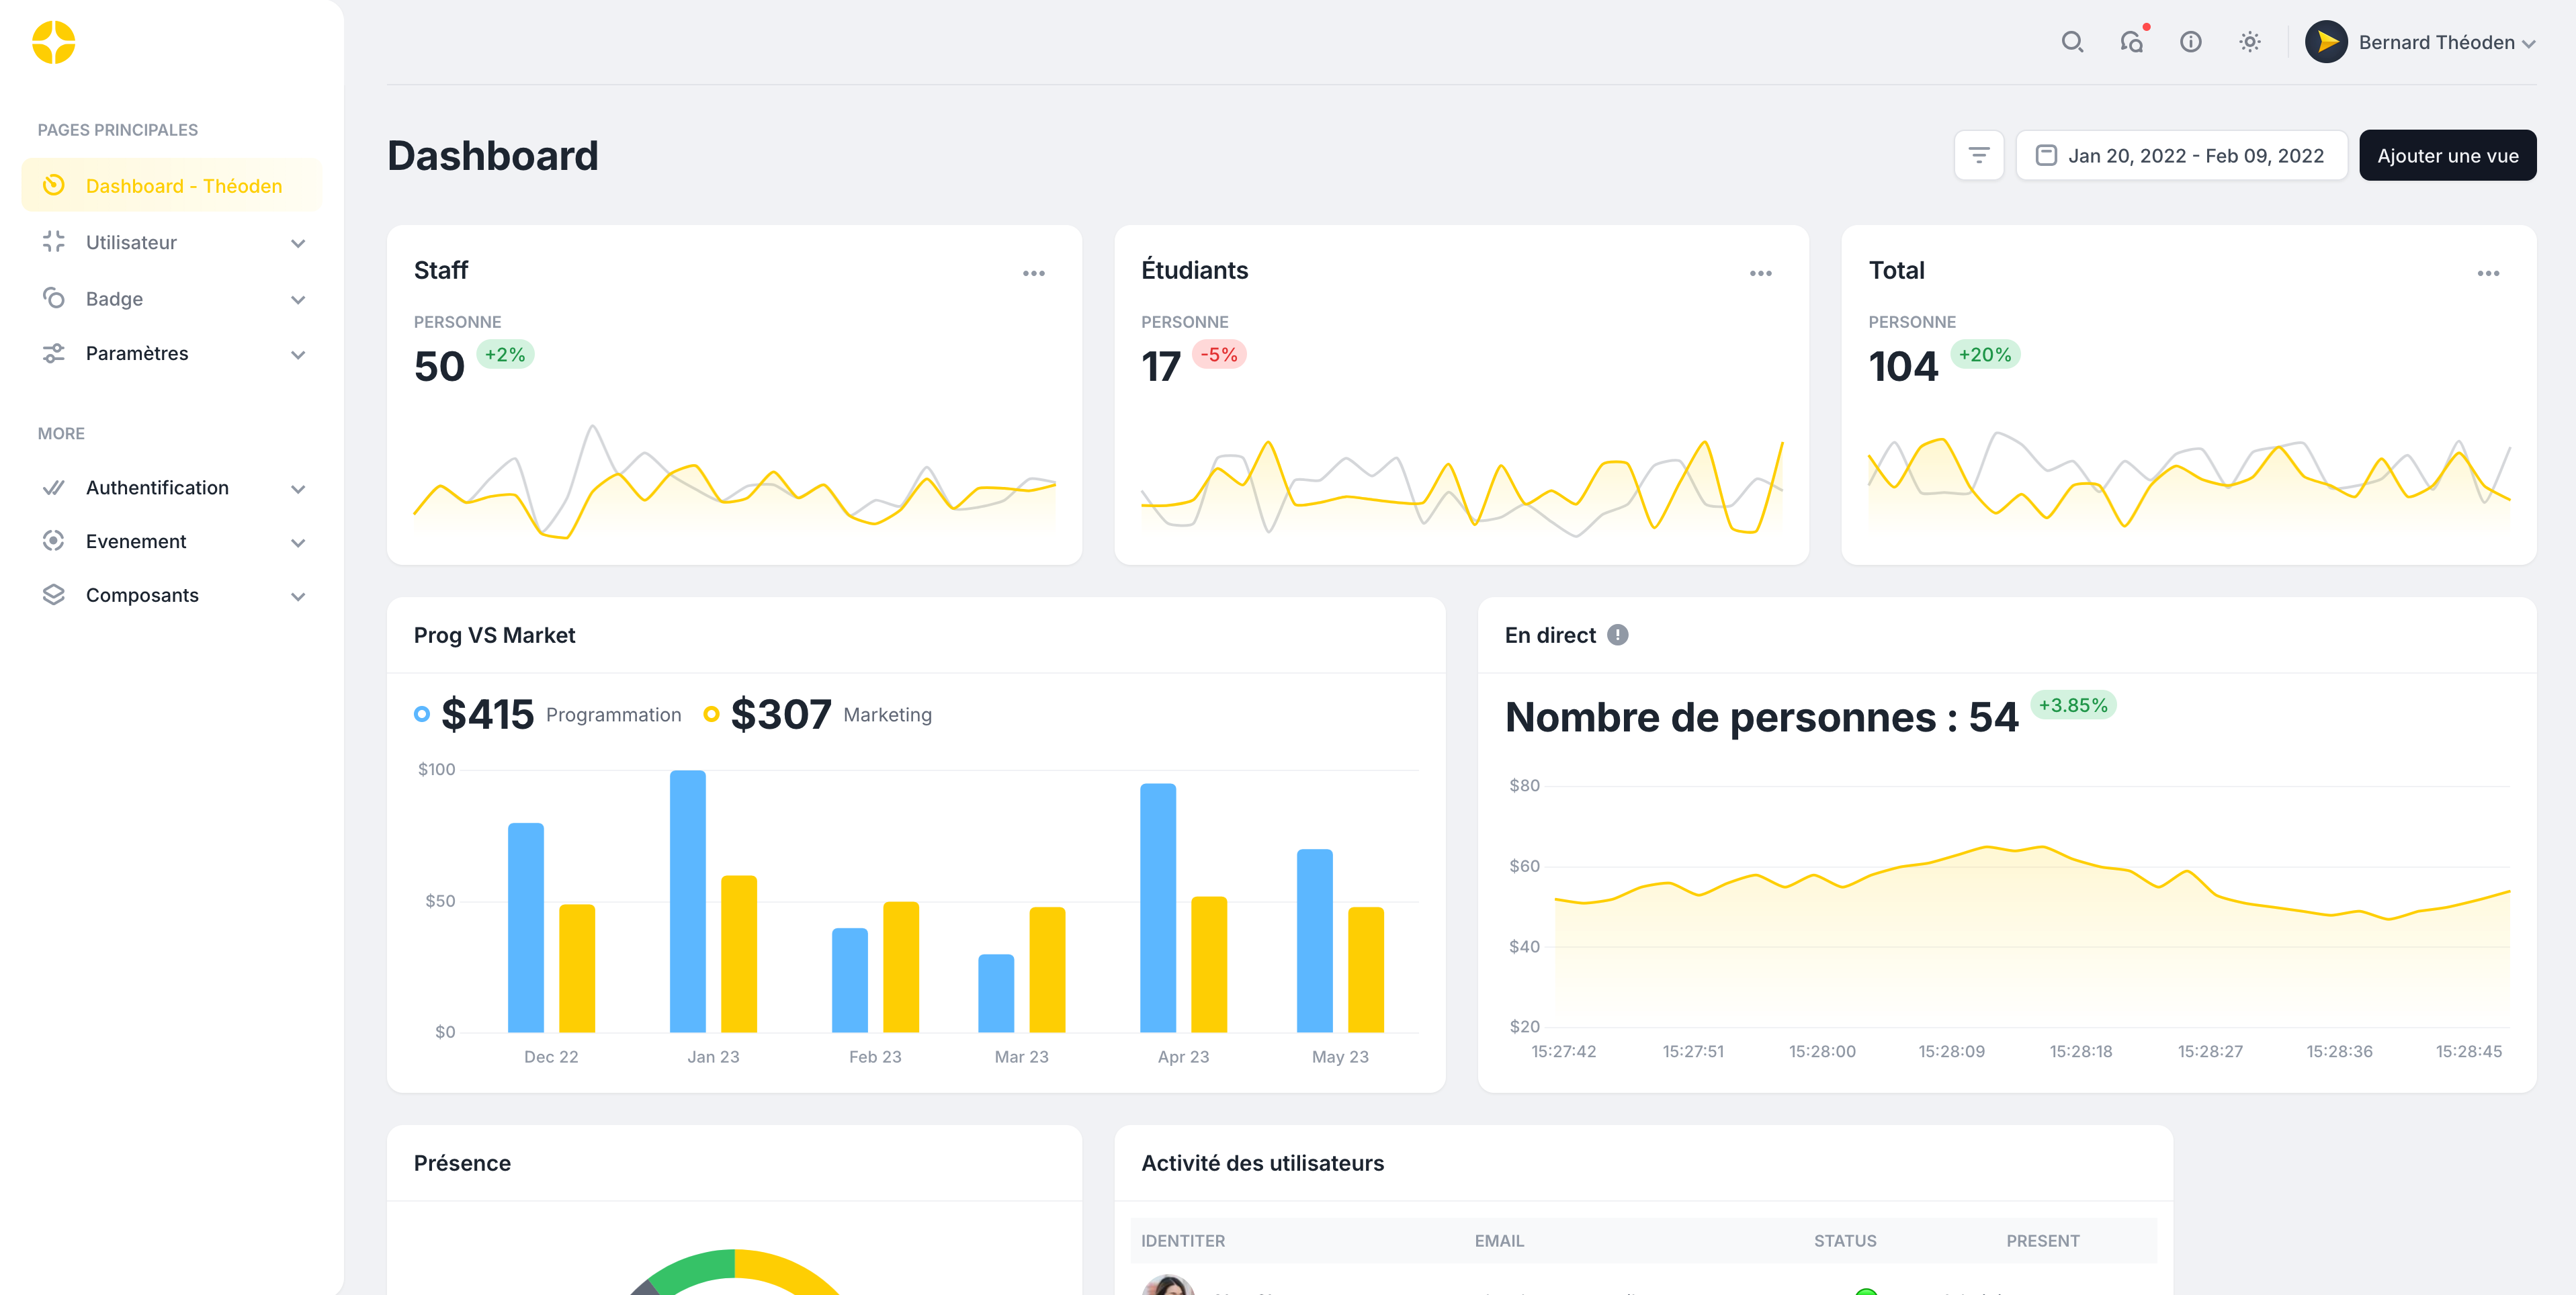
\includegraphics[width=15cm,height=80mm]{./assets/maquette/dashboard.png}
    \end{center}
\end{for_you}

\textbf{\newline}

\begin{for_you}{Page de gestions d'utilisateur}
    \begin{center}
        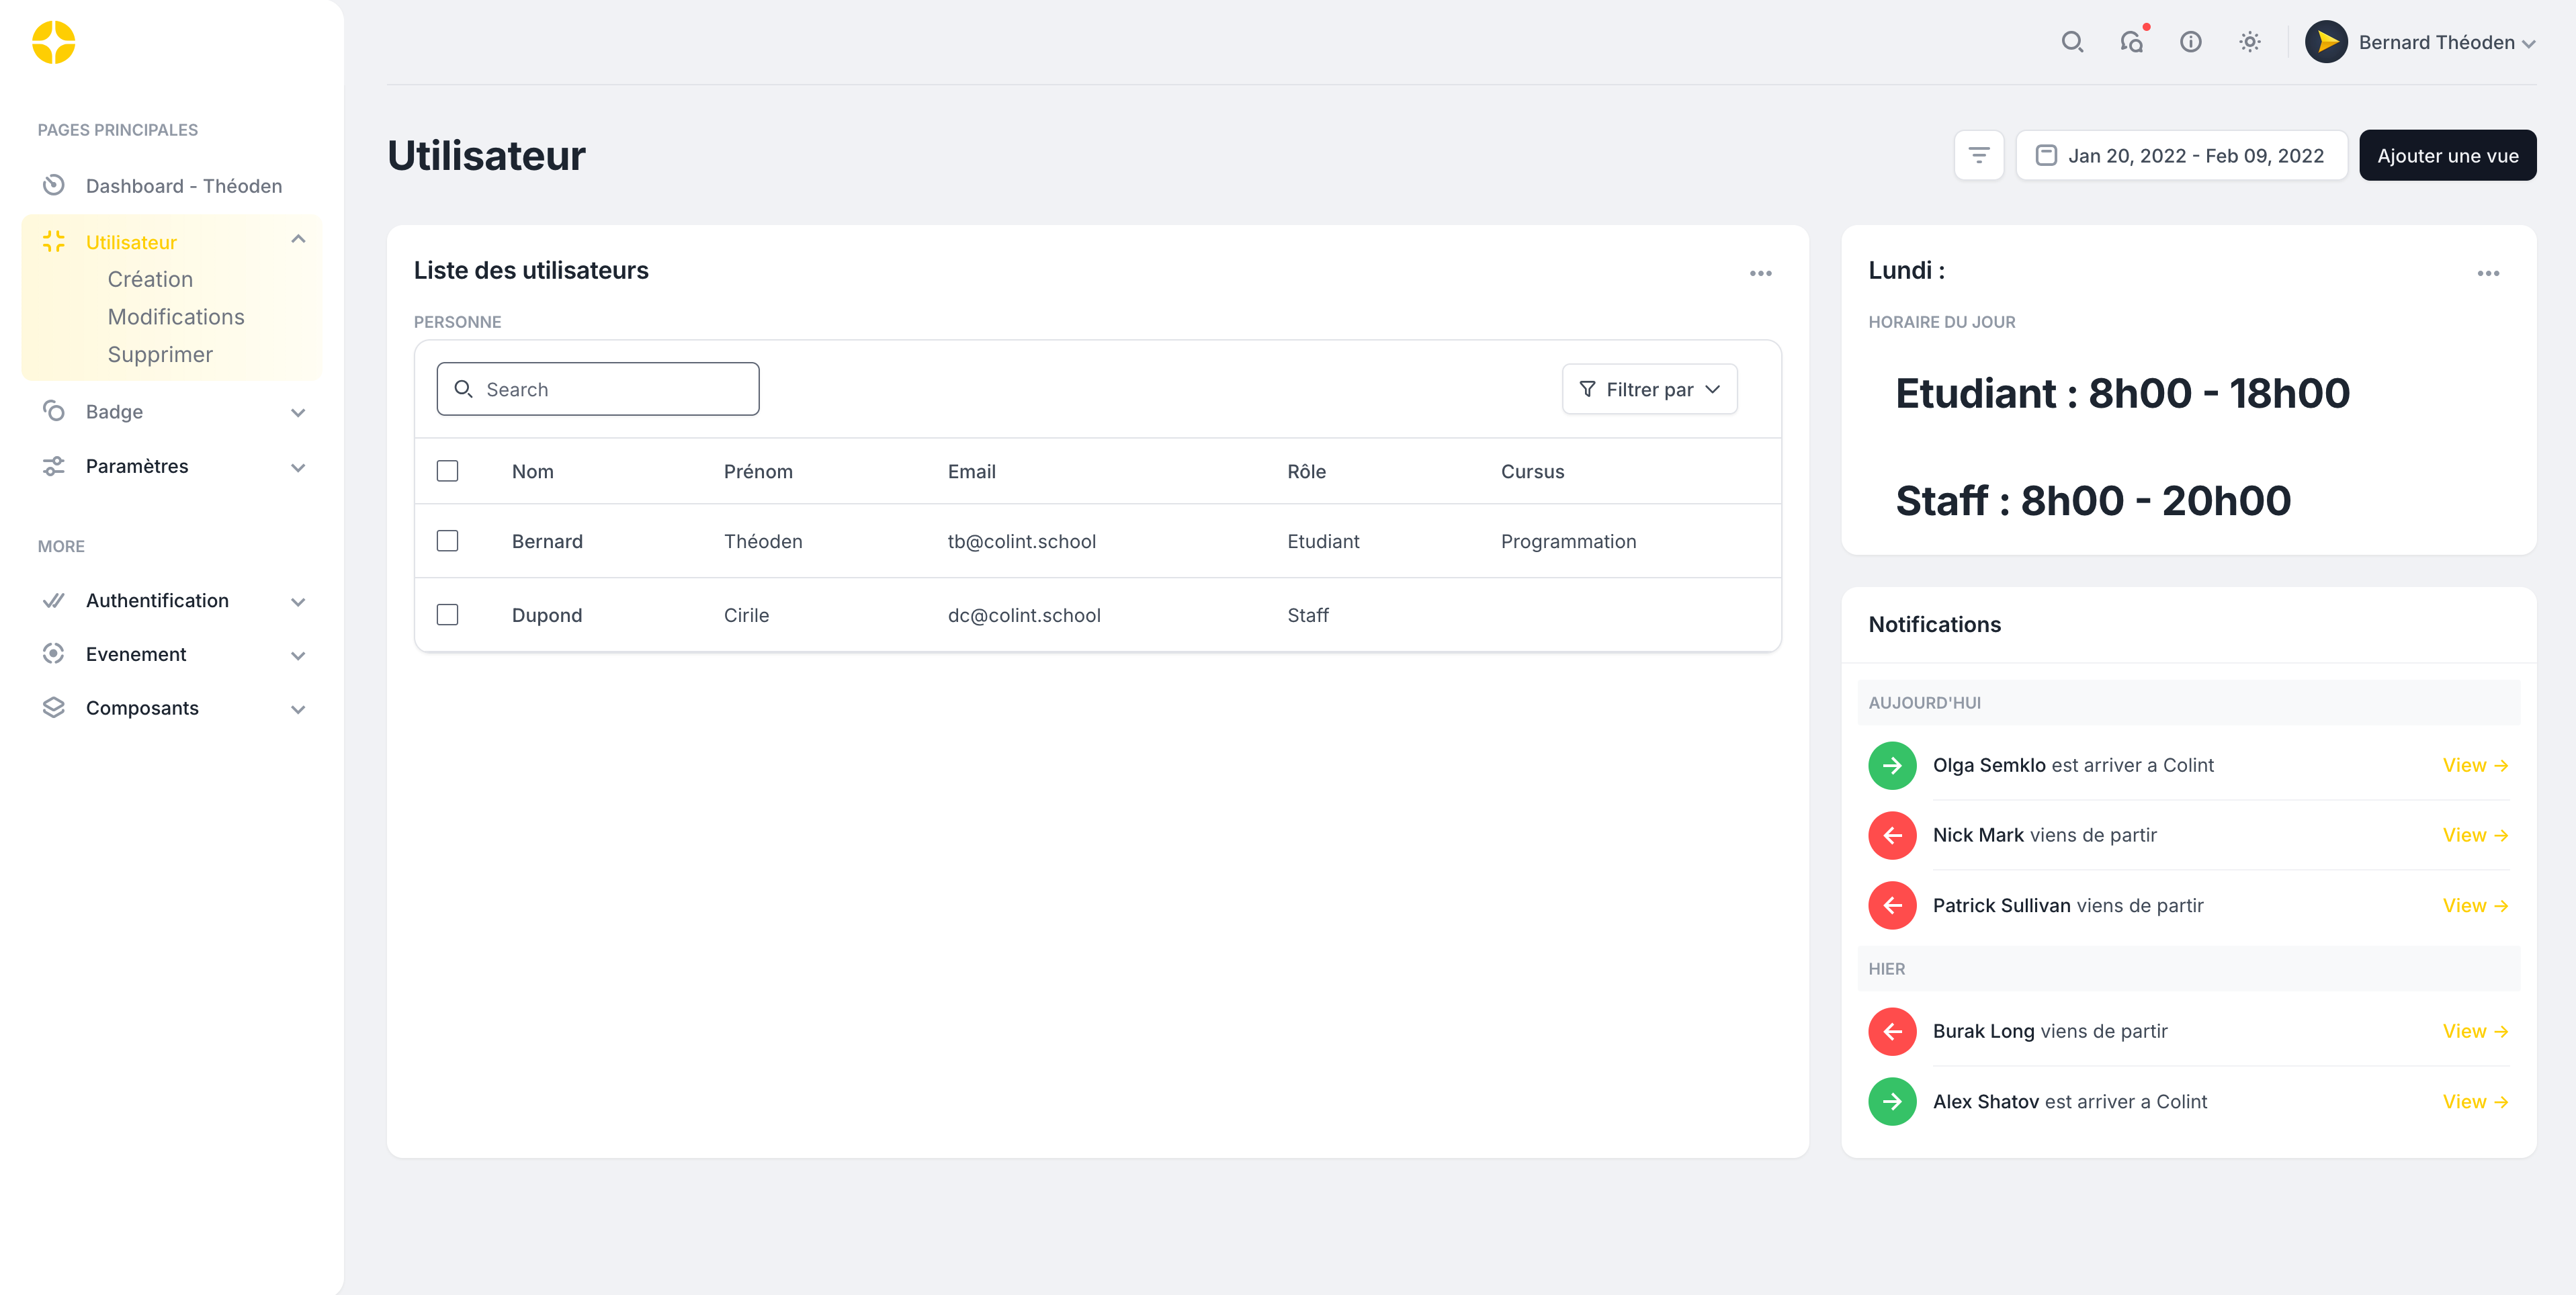
\includegraphics[width=15cm,height=80mm]{./assets/maquette/page_utilisateur.png}
    \end{center}
\end{for_you}

\textbf{\newline}

\begin{for_you}{Page de gestion de badge}
    \begin{center}
        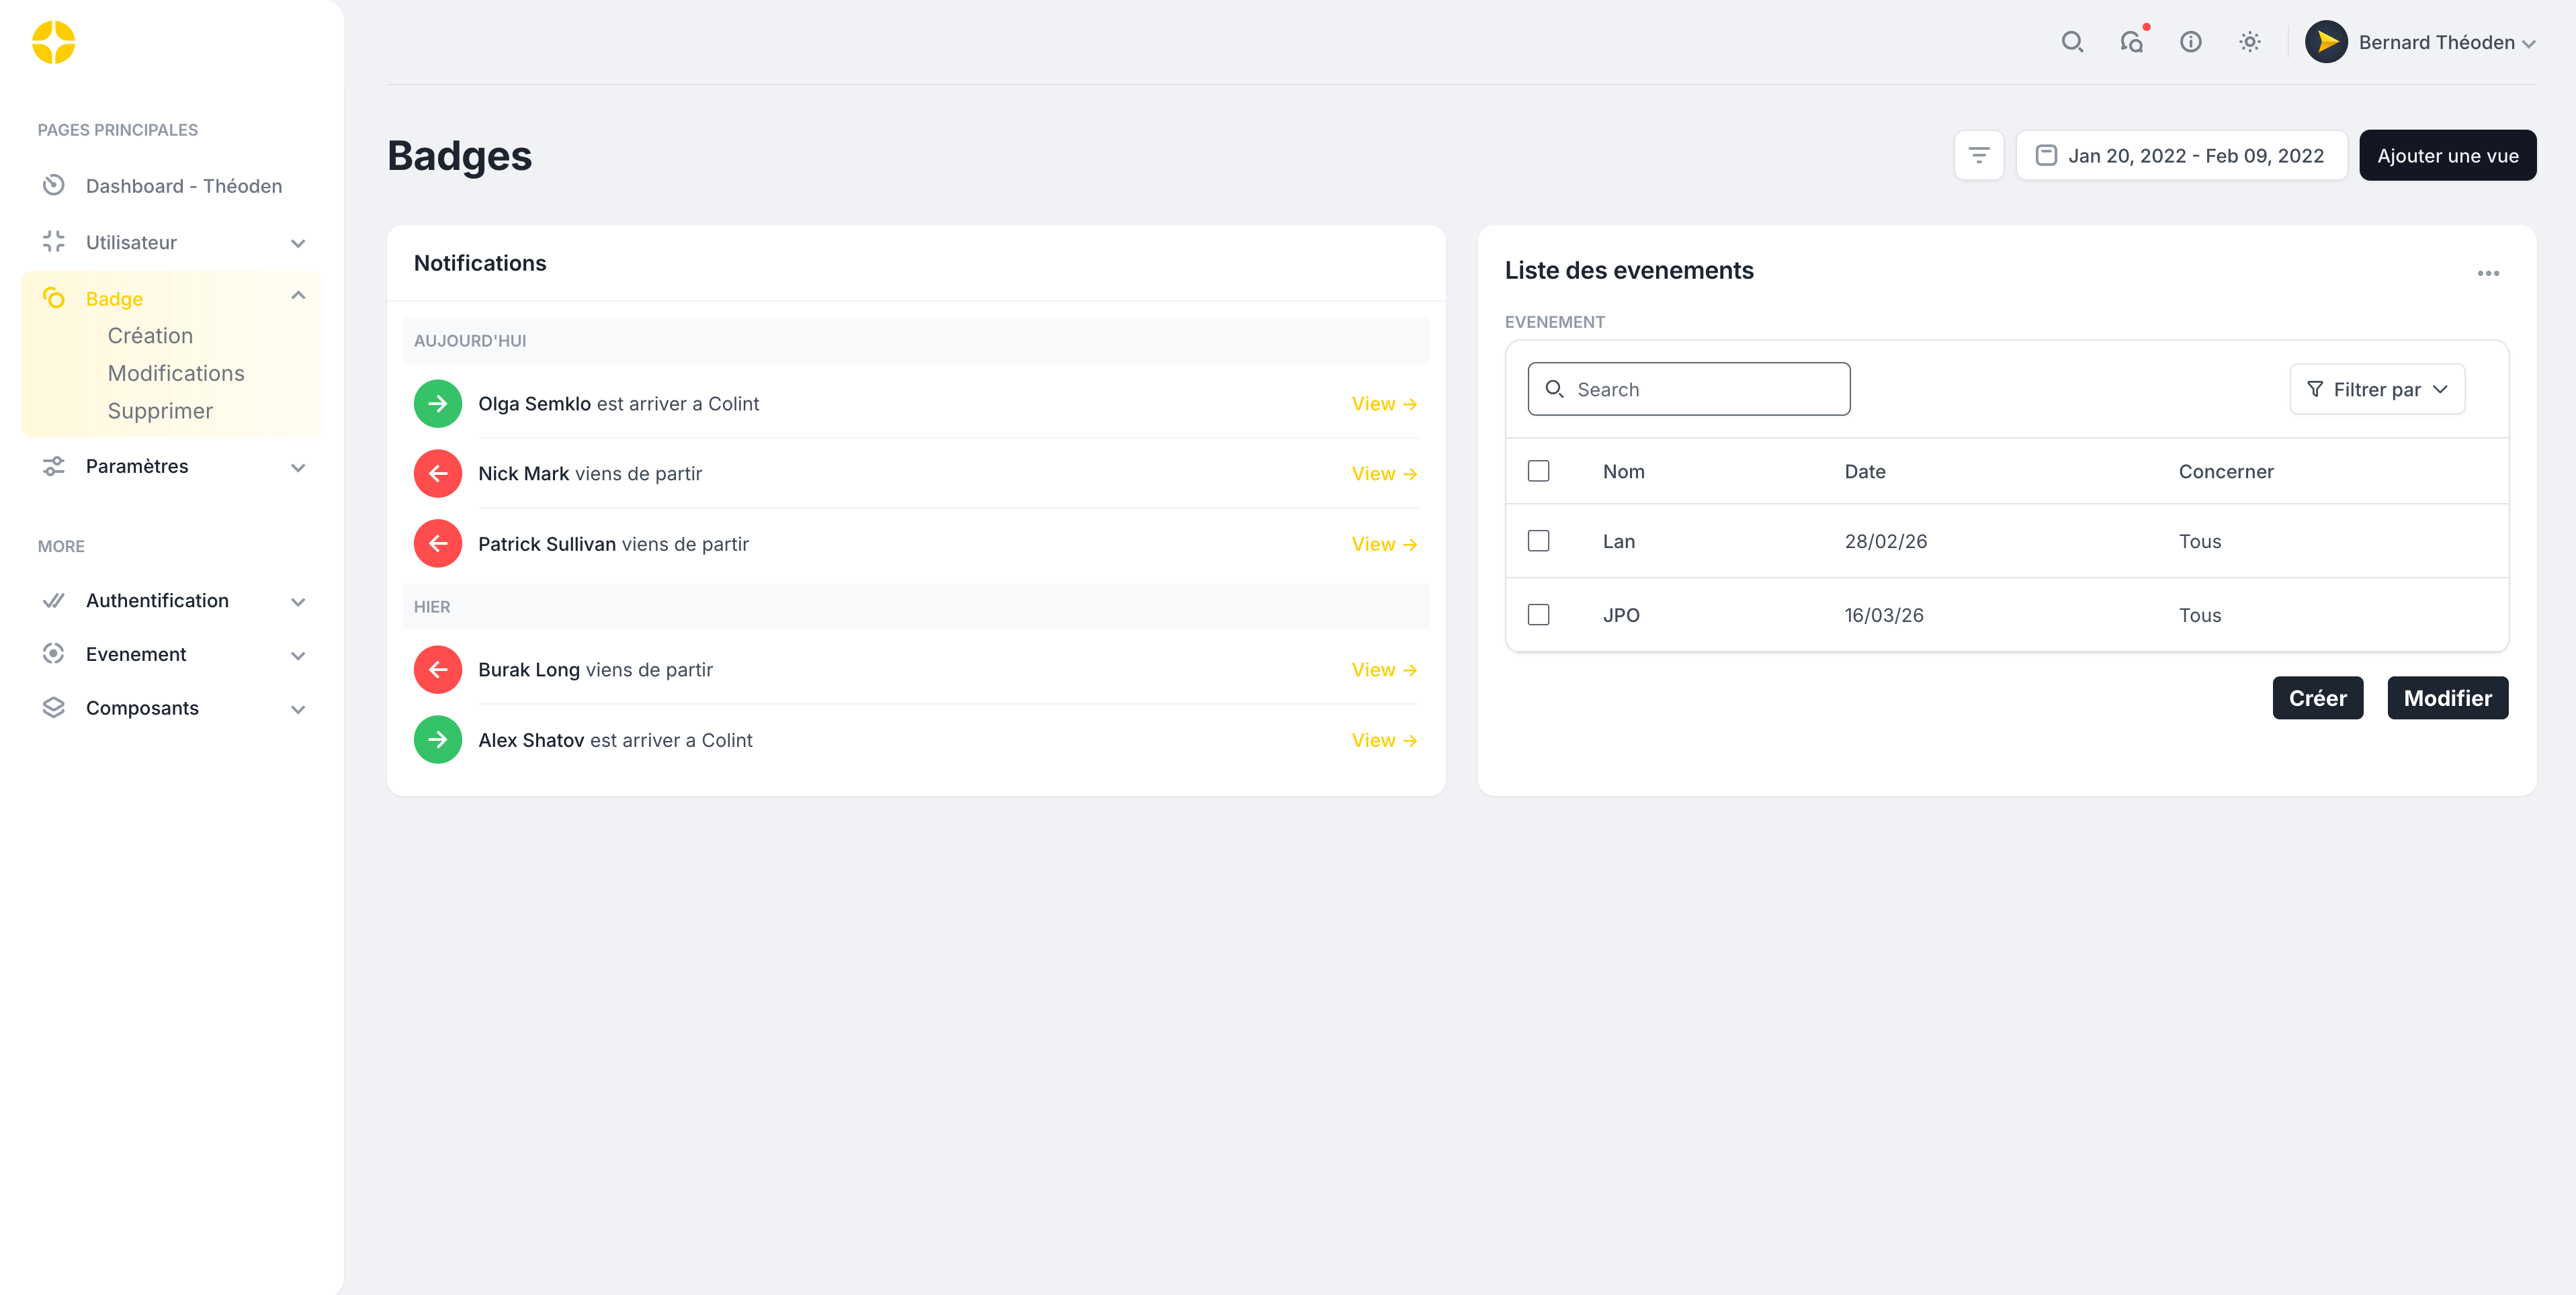
\includegraphics[width=15cm,height=80mm]{./assets/maquette/page_badge.png}
    \end{center}
\end{for_you}

\textbf{\newline}

\begin{for_you}{Page profil}
    \begin{center}
        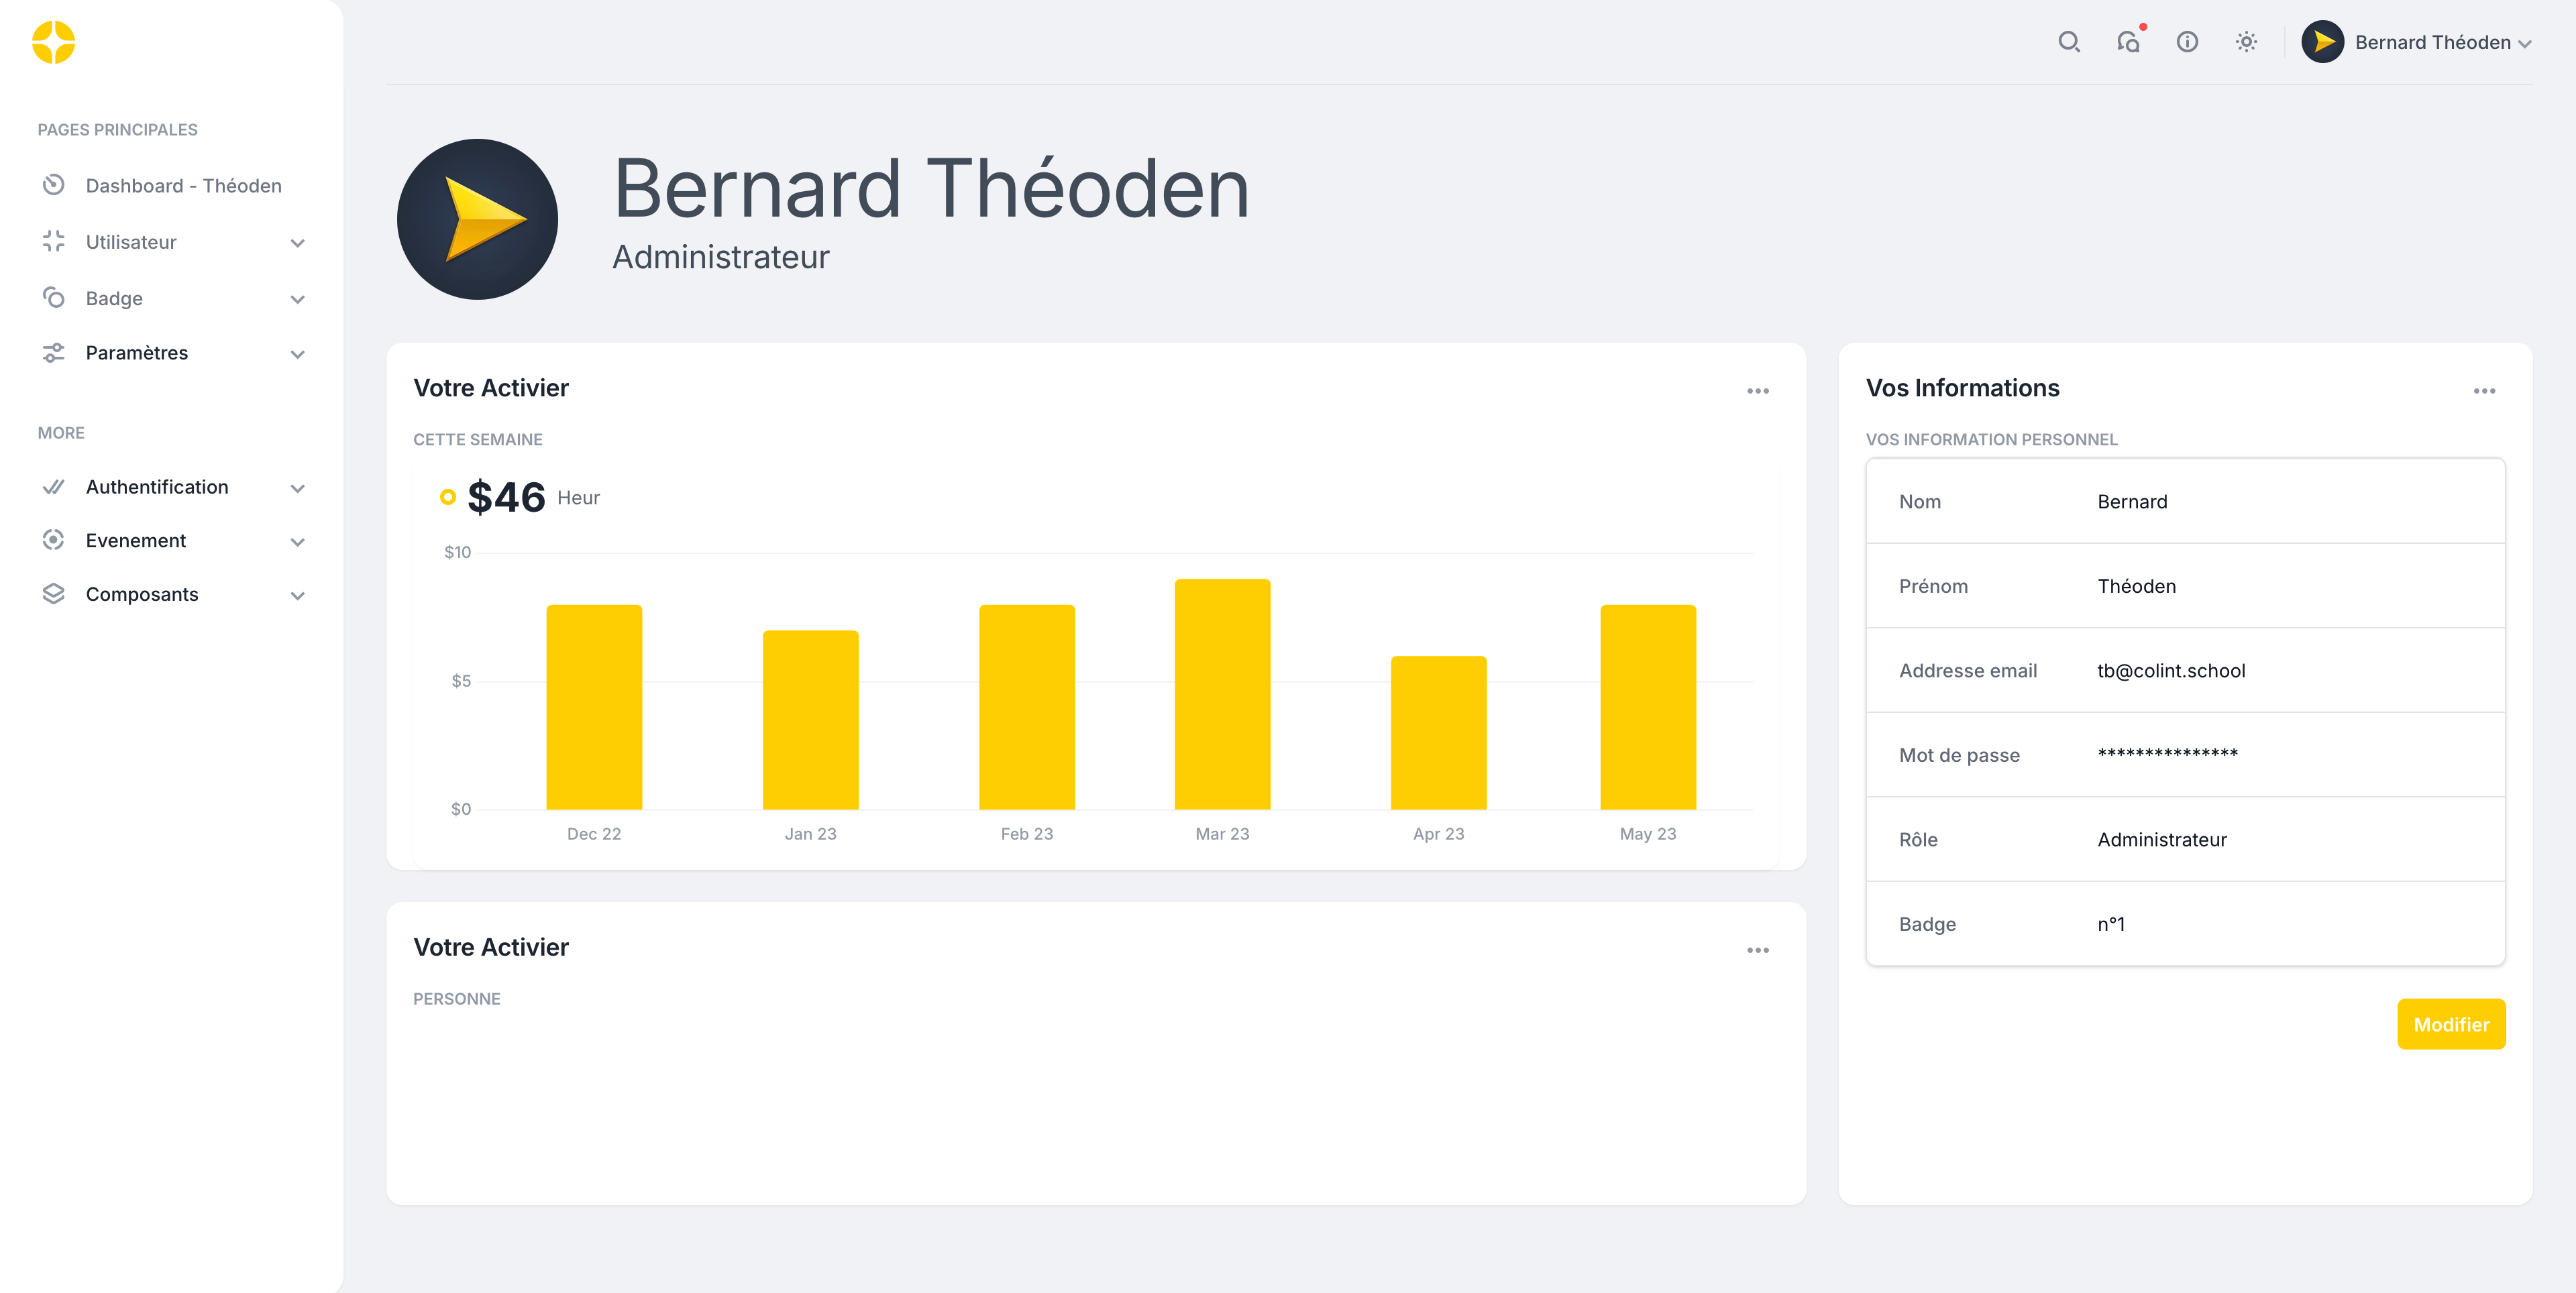
\includegraphics[width=15cm,height=80mm]{./assets/maquette/page_profil.png}
    \end{center}
\end{for_you}

\textbf{\newline}


\subsection{Outils de conception et diagrammes}

Dans cette sous-section, je vais vous présenter les outils que j'ai utilisés pour créer mes diagrammes. Nous verrons des diagrammes clairs et bien conçus qui facilitent la compréhension de votre architecture.
\newline

\textbf{Mes outils de diagrammes :} \textit{J'utilise Lucidchart ; c'est gratuit, sur internet et pratique car il dispose de beaucoup de vidéos à son sujet. De plus, il a une interface moderne qui donne envie de travailler.
\newline}

\subsection{Charte graphique}
La charte graphique garantit une cohérence visuelle sur l’ensemble des interfaces. Elle s’appuie sur l’identité de l’établissement Colint afin d’assurer une intégration future naturelle au sein de l’intranet existant.
\textit{\newline}

\begin{for_you}{Palette de couleurs :}
    \begin{itemize}
        \color{colintYellow}
        \item Jaune 
        \color{colintBlack}
        : HEX : [FFD401]

        \item Noir 
        : HEX : [000000]
        
        \color{colintWhite}
        \item Blanc
        \color{colintBlack}
        : HEX : [FFFFFF]
    \end{itemize}
\end{for_you}
\textit{\newline}

\begin{for_you}{Système typographique :}
    \textit{\newline J'utiliserai la police d'écriture \underline{Farro}}
\end{for_you}
\textit{\newline}

\begin{for_you}{Logo et son utilisation :}
    \textit{\newline Mon logo sera celui de Colint étant donné qu'il sera utilisé pour cette école et qu'il sera, dans le futur, intégré à l'intra de Colint. Il n'y aura pas de variante de ce logo.}
\end{for_you}

\textit{\newline}

\begin{for_you}{Charte graphique :}
\begin{center}
\begin{tabular}{|p{3cm}|p{4cm}|p{5cm}|}
\hline
\textbf{Couleurs} & \textbf{Typographie} & \textbf{Composants} \\
\hline
Primaire : \#FFD401 & Farro (titres) & Boutons arrondis \\
Secondaire : \#000000 & Farro (corps) & Cartes avec ombres \\
Neutre : \#FFFFFF & Monospace (code) & Icônes Material Design \\
\hline
\textbf{Espacement} & \textbf{Grille 8px} & \textbf{Marges cohérentes} \\
\hline
\end{tabular}
\end{center}
\end{for_you}

\section{Conception de la base de données}
La conception de la base de données suit la méthode Merise avec une progression structurée : Modèle Conceptuel de Données (MCD), Modèle Logique de Données (MLD) et Modèle Physique de Données (MPD).
Cette approche garantit l’intégrité des données, la cohérence des relations et l’optimisation des performances. PostgreSQL est utilisé pour sa robustesse, sa gestion stricte des contraintes et sa fiabilité transactionnelle.

\newpage
\subsection{MCD (Modèle Conceptuel de Données)}

Dans cette sous-section, je vais vous présenter mon modèle conceptuel de données. Nous verrons une représentation claire des entités et de leurs relations.
\newline

\begin{for_you}{Mon MCD :}
    \begin{center}
        
\includegraphics[width=15cm,height=80mm]{./assets/uml/mcd.png}
    \end{center}
\end{for_you}

\subsection{MLD (Modèle Logique de Données)}

Dans cette sous-section, je vais vous détailler mon modèle logique de données. Nous verrons une traduction du MCD en structure de base de données.
\newline

\begin{for_you}{Mon MLD :}
    \begin{center}
        
\includegraphics[width=15cm,height=80mm]{./assets/uml/mld.png}
    \end{center}
\end{for_you}

\newpage
\subsection{MPD (Modèle Physique de Données)}

Dans cette sous-section, je vais vous présenter mon modèle physique de données. Nous verrons une implémentation concrète avec les contraintes et index.
\newline

\begin{for_you}{Mon MPD :}
\begin{center}
    
\includegraphics[width=15cm,height=80mm]{./assets/uml/mpd.png}
\end{center}
\end{for_you}
\textit{\newline}

\begin{for_you}{Exemple de contraintes PostgreSQL :}
    \begin{lstlisting}[language=SQL]
    -- Contraintes d'intégrité
    ALTER TABLE taches ADD CONSTRAINT fk_tache_projet
        FOREIGN KEY (projet_id) REFERENCES projets(id)
        ON DELETE CASCADE;

    -- Index pour optimiser les performances
    CREATE INDEX idx_taches_statut ON taches(statut);
    CREATE INDEX idx_taches_projet_statut ON taches(projet_id, statut);

    -- Contrainte de validation
    ALTER TABLE projets ADD CONSTRAINT chk_dates
        CHECK (date_fin > date_debut);
    \end{lstlisting}
\end{for_you}

\newpage
\section{Architecture 3 tiers}
L’architecture retenue repose sur un modèle 3 tiers, séparant clairement la couche présentation (Phoenix LiveView), la logique métier (Elixir) et la couche données (PostgreSQL).
Cette séparation favorise la maintenabilité, la scalabilité et la testabilité du système. Chaque couche peut évoluer indépendamment sans impacter l’ensemble de l’architecture.
\newline

\begin{for_you}{Schéma architecture 3 tiers :}
    \begin{center}
        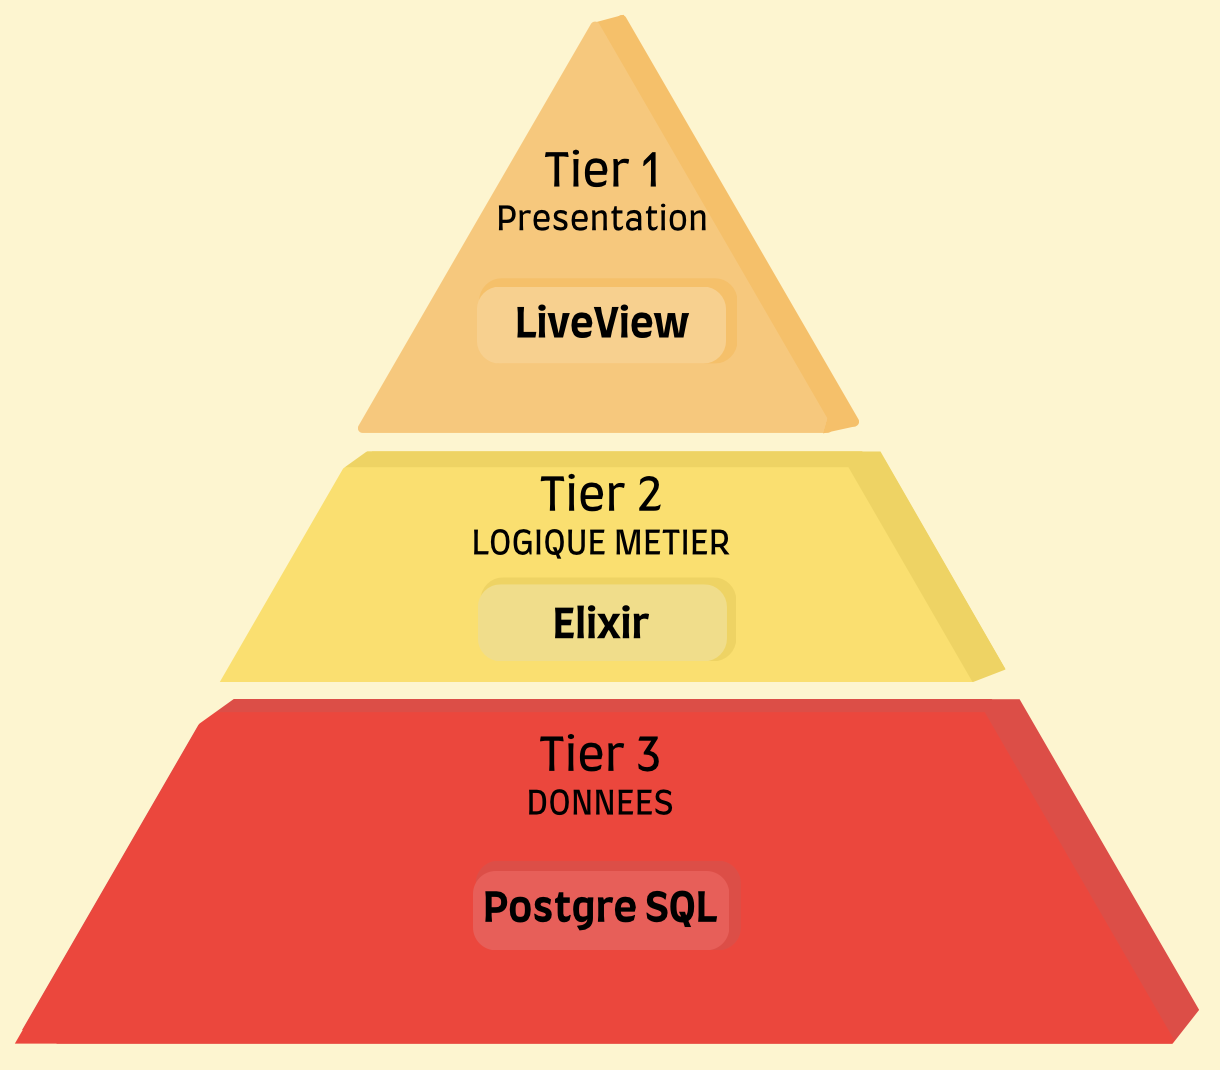
\includegraphics[width=10cm,height=80mm]{./assets/schema/architecture_3_tier.png}
    \end{center}
\end{for_you}

\section{Liens utiles}

\begin{itemize}
    \item UML: \url{https://www.uml-diagrams.org/}
    \item Merise (FR): \url{https://perso.liris.cnrs.fr/pierre-antoine.champin/enseignement/intro-merise.html}
    \item OWASP ASVS: \url{https://owasp.org/ASVS/}
    \item PostgreSQL Docs: \url{https://www.postgresql.org/docs/}
    \item MongoDB Modeling: \url{https://bit.ly/mongodb-modeling}
    \item Draw.io (diagrammes): \url{https://app.diagrams.net/}
    \item Lighthouse (accessibilité): \url{https://developers.google.com/web/tools/lighthouse}
    \item Lucidchart (UML): \url{https://www.lucidchart.com/pages/fr/exemples/diagramme-uml}
    \item PlantUML (diagrammes): \url{https://plantuml.com/}
    \item Mermaid (diagrammes): \url{https://mermaid-js.github.io/mermaid/}
\end{itemize}